\chapter{Fundamentação Teórica}

\lipsum[1-2]

\begin{citacao}
\lipsum[1]\cite[p. ~34]{Huizinga2014}
\end{citacao}

\section{Jogos Digitais}

De acordo com \citeonline{SalenZimmerman2012}, os jogos digitais...

\lipsum[4-7]

\section{Mundos Virtuais}

\lipsum[8-9]

A figura \ref{fig:kings-landing} representa \emph{King's Landing}, cenário da série \emph{Game of Thromes} reproduzido no Minecraft:

\begin{figure}[h]
	\caption{\emph{The King's Landing} no Minecraft}
	\center
	\label{fig:kings-landing}
	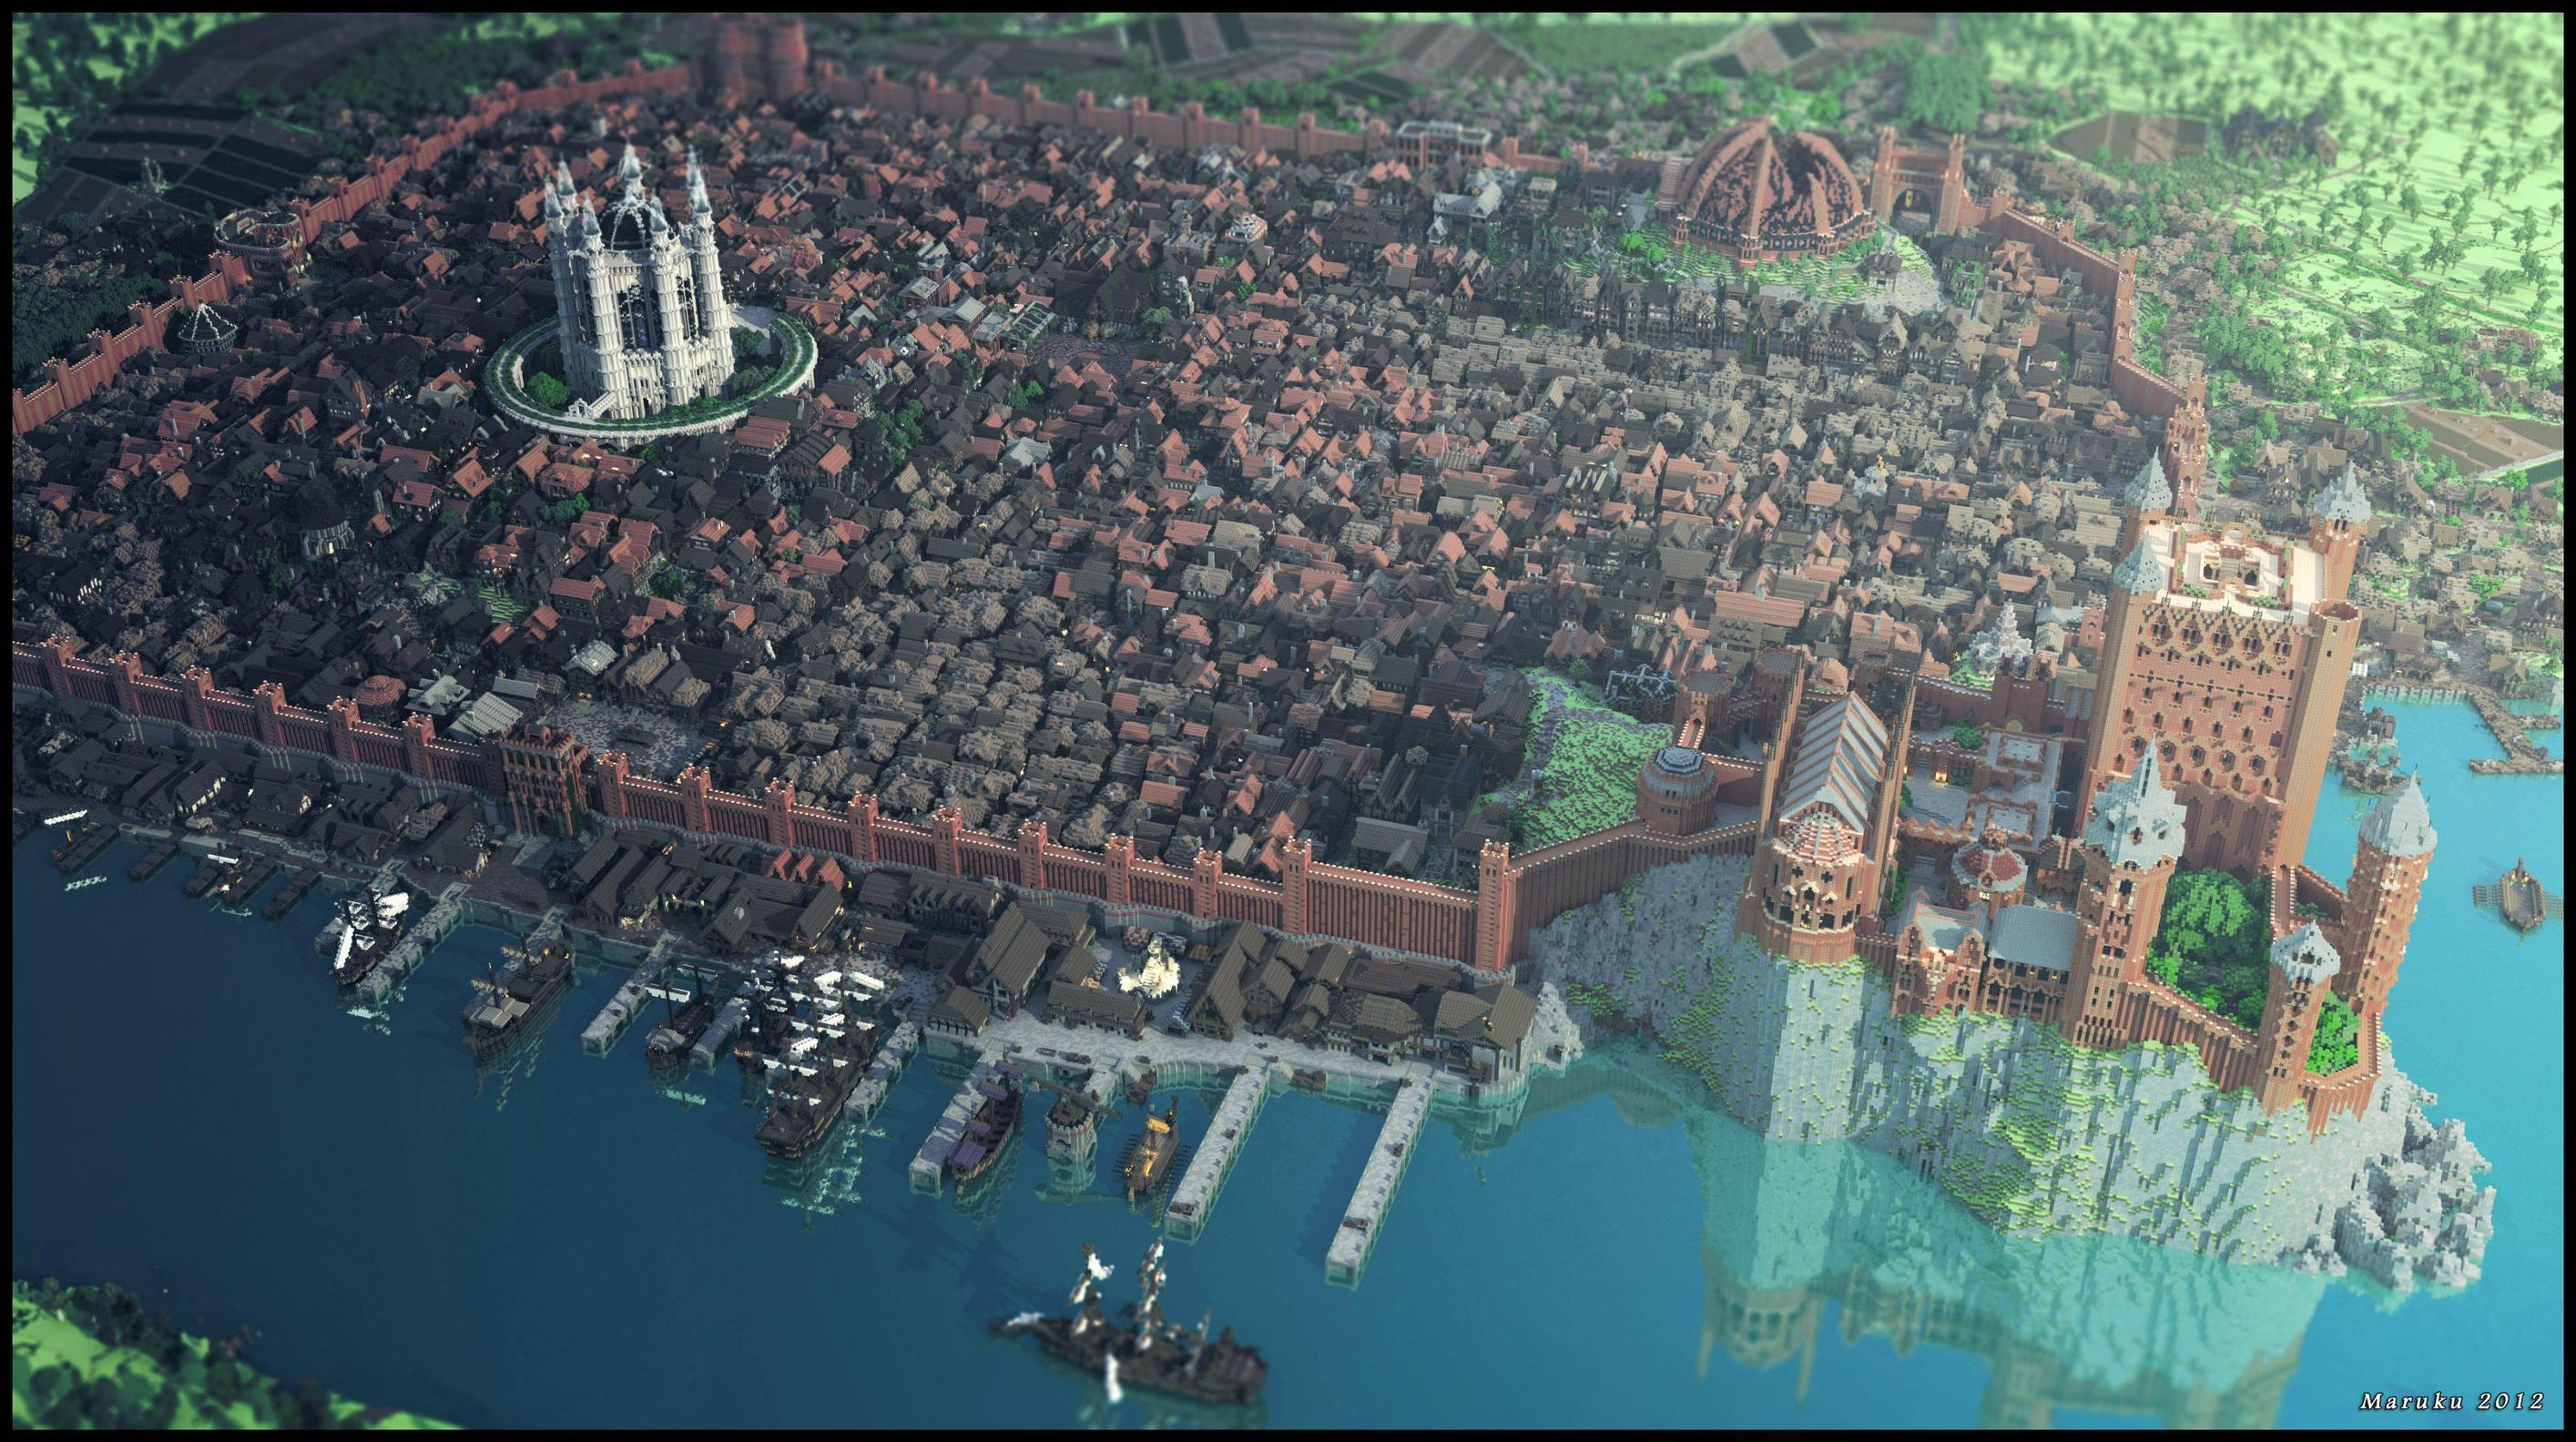
\includegraphics[scale=0.15]{fundamentacao/kings-landing.jpg}
	\fol{Imgur2013}
\end{figure}

\lipsum[10-12]

